\section{Results}
The results include 6 tables which refer back to each test performed in the Methodology above.
Tests II - V have been made into graphs for easier readability.

\subsection{Tables}

\Table{Benchmarking and Non-threaded tests and Times (ms)}{ccc}{
 & \textbf{Python} & \textbf{C} \\
 \textbf{Test} & Golden Measure & Non-threaded
}{
 \textbf{1} & 403 & 11,1 \\
 \textbf{2} & 412 & 15,1 \\
 \textbf{3} & 406 & 6,12 \\
 \textbf{4} & 367 & 7,07 \\
 \textbf{5} & 383 & 7,65 \\
 \hline
\textbf{Average} & 394 & 9,41 \\
}{Test1}

The Non-threaded C code ran 41 times faster compared to the python Golden Measure

\Table{Threaded tests and Times (ms)}{ccccccc}{
 \multicolumn{1}{c}{} & \multicolumn{6}{c}{\textbf{Threads}} \\
 \textbf{Test} & 1 & 2 & 4 & 8 & 16 & 32
}{
 \textbf{1} & 11,2 & 1,59 & 17,3 & 8,36 & 1,46 & 3,40 \\
 \textbf{2} & 10,5 & 11,2 & 6,71 & 11,3 & 8,90 & 4,88 \\
 \textbf{3} & 25,5 & 31,2 & 22,1 & 10,9 & 26,0 & 24,4 \\
 \textbf{4} & 40,4 & 37,5 & 2,59 & 11,3 & 2,07 & 17,8 \\
 \textbf{5} & 14,9 & 52,0 & 7,66 & 1,65 & 24,8 & 29,5 \\
 \hline
 \textbf{Average} & 20,5 & 26,7 & 11,3 & 8,70 & 12,6 & 16,0 \\
}{Test2}

The test run with 8 threads was the fastest, which 44 times faster than the python Golden Measure

\Table{Compiler Optimisation Flags tests and Times (ms)}{cccccccc}{
 \multicolumn{1}{c}{} & \multicolumn{7}{c}{\textbf{Optimisation Flags}} \\
 \textbf{Test} & -O0 & -O1 & -O2 & -O3 & -Ofast & -Os & -Og
}{
 \textbf{1} & 30,4 & 14,1 & 28,2 & 28,7 & 7,10 & 21,0 & 32,8 \\
 \textbf{2} & 34,7 & 33,3 & 20,9 & 26,9 & 12,3 & 5,78 & 8,92 \\
 \textbf{3} & 8,45 & 8,09 & 36,6 & 6,02 & 19,0 & 5,03 & 21,8 \\
 \textbf{4} & 12,1 & 6,19 & 5,31 & 9,71 & 5,87 & 24,2 & 6,22 \\
 \textbf{5} & 35,1 & 48,4 & 7,77 & 53,4 & 29,1 & 5,73 & 25,3 \\
 \hline
 \textbf{Average} & 24,2 & 22,0 & 19,8 & 24,9 & 14,7 & 12,3 & 19,0 \\
}{Test3}

The test run with the \textit{-Os} flag was the fastest, which ran 31 times faster than the python Golden Measure

\Table{COFs with \textit{-funroll-loops} tests and Times (ms)}{ccccc}{
 \multicolumn{1}{c}{} & \multicolumn{4}{c}{\textbf{Optimisation Flags}} \\
 \textbf{Test} & -O0 & -O3 & -Ofast & -Os
}{
 \textbf{1} & 43,9 & 7,31 & 24,6 & 6,01 \\
 \textbf{2} & 6,18 & 6,78 & 5,08 & 5,67 \\
 \textbf{3} & 12,1 & 15,1 & 42,7 & 11,8 \\
 \textbf{4} & 31,7 & 57,9 & 6,06 & 21,1 \\
 \textbf{5} & 13,4 & 34,0 & 6,21 & 5,47 \\
 \hline
 \textbf{Average} & 21,5 & 24,2 & 16,9 & 10,0 \\
}{Test4}

The test run with \textit{-Os} and \textit{-funroll-loops} flags was the fastest, which ran 38 times faster than the python Golden Measure.
The biggest improvement when adding the \textit{-funroll-loops} flag was also the \textit{-Os} flag, with a 23\% improvement

\Table{C Bit Widths tests and Times (ms)}{cccc}{
 \multicolumn{1}{c}{} & \multicolumn{3}{c}{\textbf{Data type}} \\
 \textbf{Test} & double & float & \textunderscore \textunderscore fp16
}{
 \textbf{1} & 31,9 & 6,69 & 110 \\
 \textbf{2} & 39,2 & 31,1 & 101 \\
 \textbf{3} & 34,1 & 10,9 & 26,2 \\
 \textbf{4} & 69,0 & 35,0 & 98,8 \\
 \textbf{5} & 12,1 & 7,87 & 93,8 \\
 \hline
 \textbf{Bit widths} & 64 & 32 & 16 \\
 \textbf{Average} & 37,3 & 18,3 & 86,0 \\
}{Test5}

The test run with \textit{float} data type was the fastest, which ran 21 times faster than the python Golden Measure

\Table{Fastest Test}{cc|cc}{
 \textbf{Section} & \textbf{Fastest} & \textbf{Test} & \textbf{Time (ms)}
}{
 \textbf{Language} & C & \textbf{1} & 14,3 \\
 \textbf{Threaded} & True & \textbf{2} & 1,68 \\
 \textbf{Threads} & 8 & \textbf{3} & 14,6 \\
 \textbf{Compiler Flag} & -Os & \textbf{4} & 1,90 \\
 \textbf{Unroll loops} & True & \textbf{5} & 21,7 \\
 \cline{3-4}
 \textbf{Data type} & float & \textbf{Average} & 10,8 \\
}{Test6}

It should be noted that the data was extremely variable throughout all the tests and an average of 5 samples was likely to few for accurate testing.

\subsection{Figures}

\begin{figure}[htd]
 \centering
 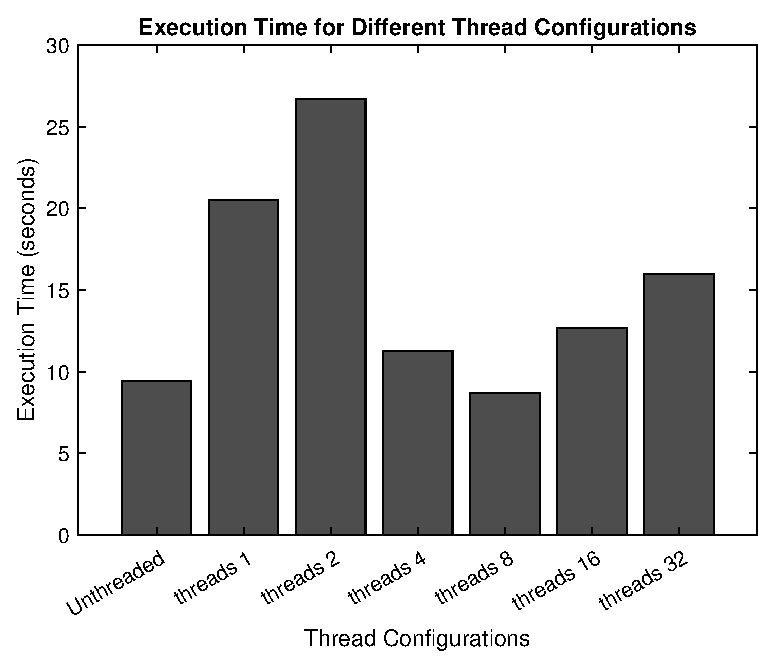
\includegraphics[width=0.5\textwidth]{bargraf_on_C_Threaded}
 \caption{Bar graph representing different C threading configurations.}
 \label{fig:threading}
\end{figure}


